

\fancypagestyle{miEstilo5}{
   \lhead{5. Descripción de la aplicación}
   %\chead{1. Introducción}
   \rhead{Página \thepage}
   \lfoot{}
   \cfoot{}
   \rfoot{}
}

\pagestyle{miEstilo5}

\section{Descripción de la aplicación: SIVIRA}

El sistema de videovigilancia con una Raspberry PI (\texttt{SIVIRA}) es una aplicación que nos permite construir un sistema de seguridad basado en la videovigilancia de bajo coste utilizando una Raspberry PI , una cámara y un sensor de movimiento.

La idea es poder controlar el sistema a través de una aplicación móvil, con la que el usuario pueda conectarse desde cualquier parte y tener acceso a su información y sistema de seguridad. Las funciones principales de este sistema son las siguientes:

\begin{itemize}
\item \textbf{Sistema automático} de alertas generadas al capturar el movimiento.
\item \textbf{Sistema manual} para grabar vídeo o capturar una foto instantáneamente.   
\item \textbf{Sistema de streaming} para visualizar la imagen en tiempo real.
\end{itemize}

Además, podemos realizar configuraciones personalizadas a la cámara, como por ejemplo, cambiar la resolución, rotación... y la opción de poder activar un agente que filtre las alertas automáticas, generando únicamente alertas cuando se detecta a una persona en una imagen (evitar falsos positivos).

\subsection{Arquitectura de la aplicación}

Esta aplicación consta de una \textbf{arquitectura basada en microservicios}. Una arquitectura de microservicios \cite{ref25} consta de una colección de servicios autónomos y pequeños. Los servicios son independientes entre sí y cada uno debe implementar una funcionalidad de negocio individual.

En cierto modo, los microservicios son la evolución natural de las arquitecturas orientadas a servicios aunque con ciertas diferencias.

\newpage

\textbf{¿Por qué se ha utilizado esta arquitectura?}

En primer lugar, se ha realizado una descomposición de los principales componentes necesarios para construir la aplicación, y se ha observado que hay funcionalidades independientes que se pueden comunicar entre sí para integrarse en la aplicación. Esto aporta una gran serie de ventajas respecto a un diseño monolítico \cite{ref26} como las siguientes:

\begin{itemize}
\item \textbf{Implementaciones independientes}: Es posible actualizar un servicio sin volver a implementar toda la aplicación y revertir o poner al día una actualización si algo va mal. Las correcciones de errores y las publicaciones de características son más fáciles de administrar y entrañan menos riesgo, por lo tanto, facilitan el mantenimiento de este software.

\item \textbf{Desarrollo independiente}: Cada microservicio se ha ido desarrollando a lo largo de una iteración y de forma independiente al resto. Esto ha agilizado bastante la tarea, ya que las modificaciones y errores no se retropropagaban.

\item \textbf{Fácil escalabilidad}: Cada microservicio puede ser escalado de forma independiente al resto. Por ejemplo, en el caso de que sea necesario escalar la detección de objetos en imágenes, bastaría con replicar el microservicio de detección de objetos y balancear las peticiones entre ellos.

\item \textbf{Fácil integración y alta cohesión}: Un sistema de microservicios se puede integrar y adaptar a casi cualquier sistema. Por ejemplo, en el caso de que quisiera añadir un sistema multicámara a la aplicación, bastaría con añadir una nueva capa superior de abstracción sobre el software desarrollado y se integraría perfectamente.
\end{itemize}

Basándome en esta arquitectura basada en microservicios, se ha diseñado el siguiente sistema (ver figura \ref{img:arquitectura}).

\newpage

\begin{figure}[h]
	\centering
	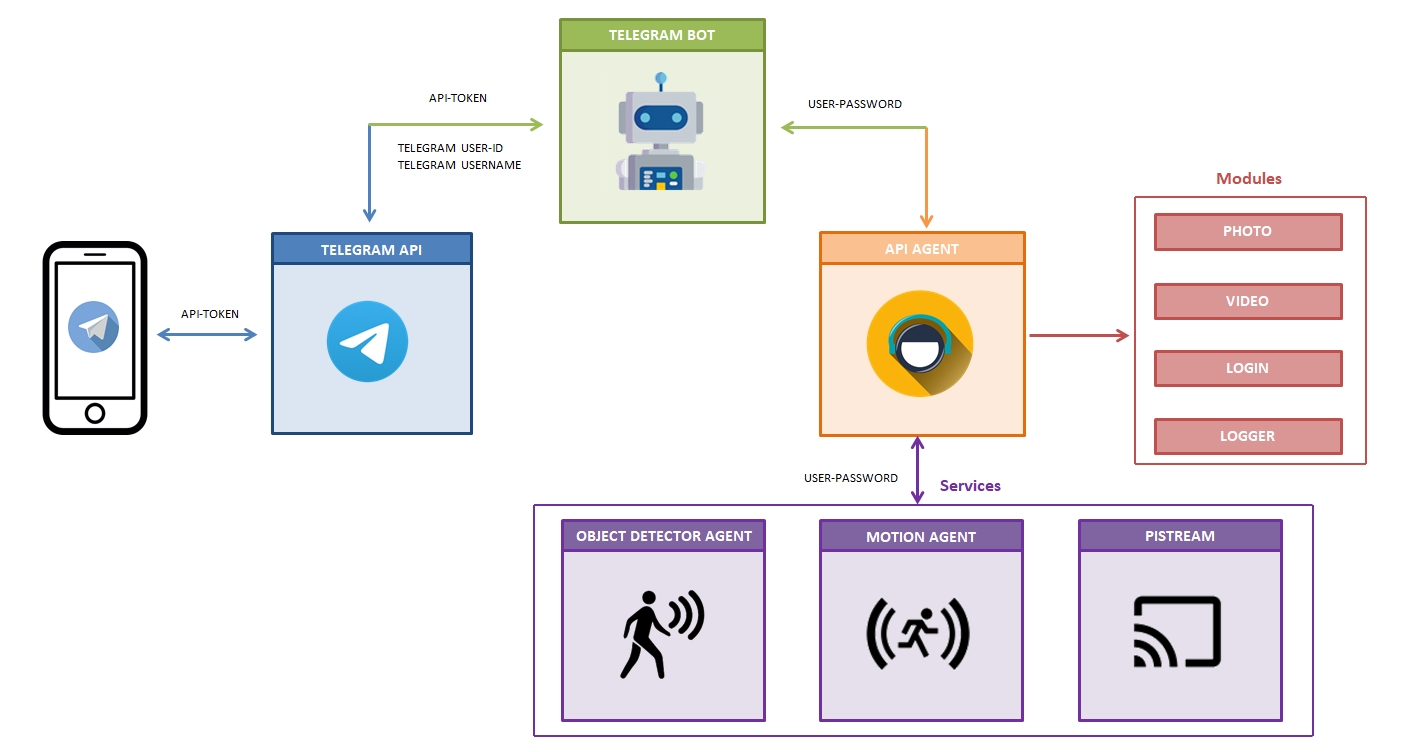
\includegraphics[scale=0.4]{images/23}
	\caption{Arquitectura de la aplicación}
	\label{img:arquitectura}
\end{figure}

En primer lugar tenemos los \textbf{módulos} de la aplicación (ver figura \ref{img:modulos}) que implementan un conjunto de funcionalidades para comunicarse con el módulo hardware de la cámara de la Raspberry PI, autenticación y logs.

\begin{figure}[h]
	\centering
	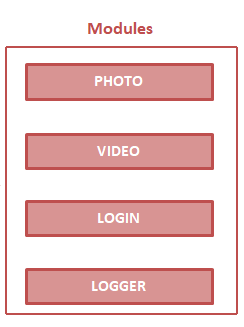
\includegraphics[scale=0.4]{images/24}
	\caption{Módulos de la aplicación}
	\label{img:modulos}
\end{figure}

A continuación tenemos el \textbf{API agent} (ver figura \ref{img:api}). Este es un servicio web que inicia la API que conecta con el resto de módulos de la aplicación.

\begin{figure}[h]
	\centering
	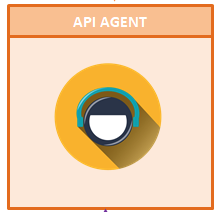
\includegraphics[scale=0.35]{images/25}
	\caption{API agent}
	\label{img:api}
\end{figure}

\newpage

Esta API importa y hace uso de los módulos de la aplicación. 

\begin{figure}[h]
	\centering
	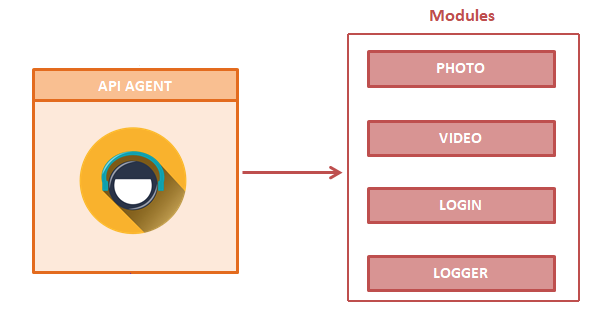
\includegraphics[scale=0.35]{images/27}
	\caption{Conexión entre la API y los módulos}
	\label{img:conexionapimodulos}
\end{figure}

Por otra parte, tenemos un conjunto de servicios que se inician de forma independiente y proporcionan las funcionalidades de detección de objetos en imágenes, detección de movimiento y servicio de streaming.

\begin{figure}[h]
	\centering
	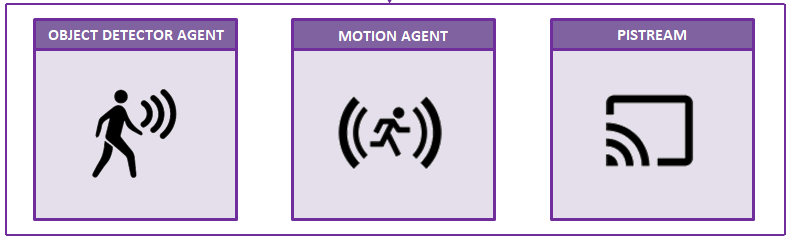
\includegraphics[scale=0.35]{images/26}
	\caption{Servicios de la aplicación}
	\label{img:serviciosaplicacion}
\end{figure}

La API está conectada con todo este conjunto de servicios y tiene la capacidad de poder gestionarlos.

\begin{figure}[h]
	\centering
	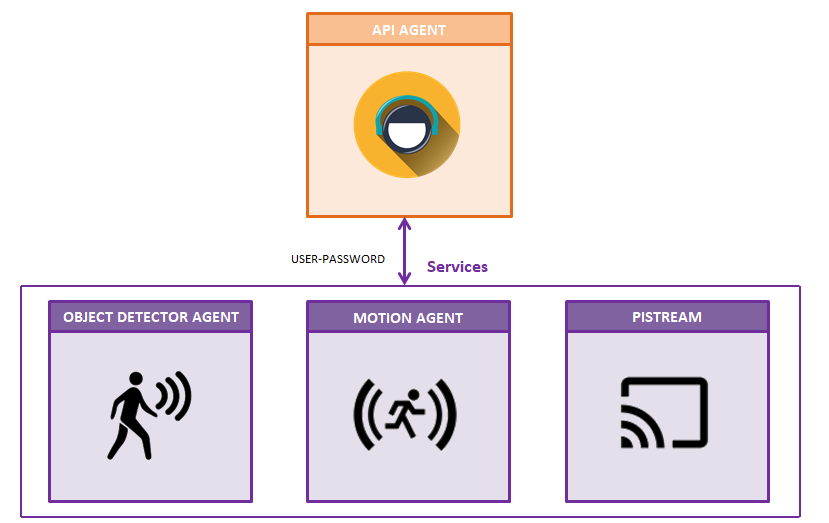
\includegraphics[scale=0.35]{images/28}
	\caption{Conexión entre los servicios y la API}
	\label{img:conexionserviciosapi}
\end{figure}

En la figura \ref{img:conexionmodulosserviciosapi} podemos ver, como quedan unidos todos estos componentes entre sí.

\newpage


\begin{figure}[h]
	\centering
	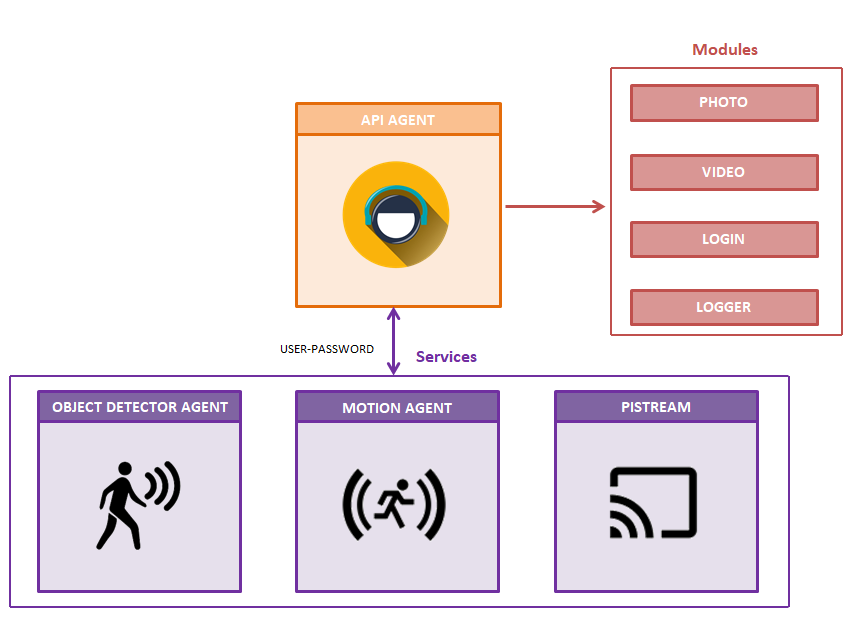
\includegraphics[scale=0.35]{images/35}
	\caption{Conexión de módulos y servicios con la API}
	\label{img:conexionmodulosserviciosapi}
\end{figure}

El siguiente componente es el \textbf{bot de Telegram}. Este bot es un proceso que se ejecuta junto a la API, cuyo objetivo es conectar la API de telegram con la API de la aplicación.

\begin{figure}[h]
	\centering
	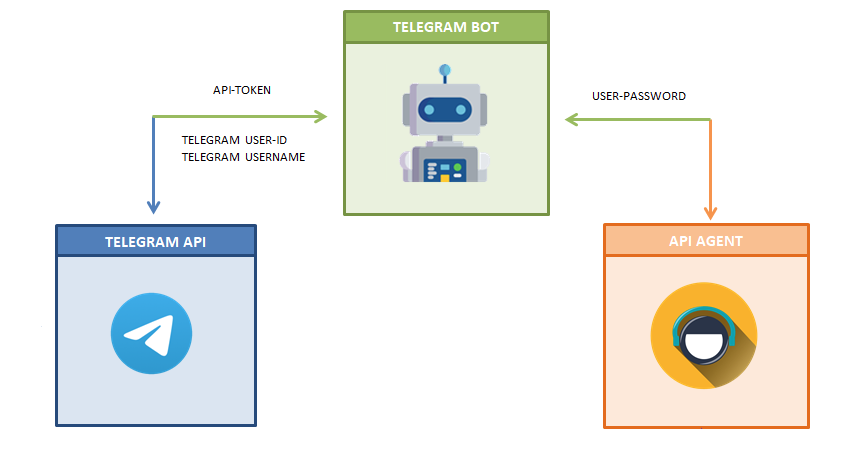
\includegraphics[scale=0.35]{images/34}
	\caption{Conexión entre el bot de telegram y la API}
	\label{img:conexionbotapitelegram}
\end{figure}

Finalmente, el usuario puede interactuar con la aplicación (\texttt{SIVIRA}), haciendo uso de la aplicación multiplataforma \texttt{Telegram}, usando el bot que se ha creado.

\begin{figure}[h]
	\centering
	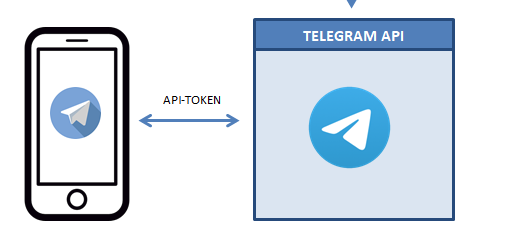
\includegraphics[scale=0.35]{images/33}
	\caption{Conexión entre el usuario y la aplicación}
	\label{img:usuariotelegram}
\end{figure}

\newpage

\subsection{Descripción de los componentes}

La aplicación (SIVIRA) desarrollada en este proyecto está compuesta por los siguientes componentes:

\subsubsection{Módulos}

Los módulos son un conjunto de funciones cuyo objetivo es encapsular funcionalidades que después serán utilizadas por el resto de componentes de la aplicación (ver figura \ref{img:modulos}). A continuación se realiza una descripción de cada uno de ellos.

\textbf{Logger}

Módulo cuyo objetivo es poder capturar y almacenar los logs de la aplicación en ficheros independientes para monitorizar el estado de la aplicación. Su implementación parte de una clase abstracta base, cuyo objetivo es definir las propiedades y métodos que tendrán todas las clases que implementarán los logs del sistema. 


PONER AQUÍ DIAGRAMA DE CLASES DE LOGS

\newpage

Por defecto, los logs son mostrados y almacenados de la siguiente forma:

\begin{itemize}
\item \textbf{Consola}: Corresponde a la salida \texttt{stdout}. Todo logs por encima de un nivel determinado de prioridad será mostrado por la salida de consola.

\item \textbf{Archivo de módulo}: Cada módulo y microservicio tendrán un fichero de log independiente para poder monitorizar su comportamiento a lo largo de su ejecución.

\item \textbf{Archivo de la aplicación}: La aplicación consta de un archivo de logs donde se almacenan todos los logs de módulos y microservicios de forma conjunta.

\item \textbf{Archivo de errores}: Todos los errores que surjan en cualquier módulo o microservicio es almacenado en este fichero para poder comprobar el estado de la aplicación.

\end{itemize}

Los niveles de logs que se han establecido son los siguientes:

\begin{itemize}

\item \textbf{DEBUG}: Nivel destinado a la depuración del código. Este nivel solo genera log en la salida por pantalla, y no se almacena en ningún fichero.

\item \textbf{INFO}: Nivel destinado a mostrar un mensaje informativo sobre alguna acción llevada a cabo. Estos logs son almacenados en el fichero de módulo correspondiente, en el fichero de logs de la aplicación y mostrados por pantalla.

\item \textbf{WARNING}: Nivel destinado a mostrar un mensajes de advertencia por posible mal uso de las llamadas a funciones, o simplemente porque algunas de ellas están '{deprecated}`. Estos logs son almacenados en el fichero de módulo correspondiente, en el fichero de logs de la aplicación y mostrados por pantalla.

\item \textbf{ERROR}: Nivel destinado a mostrar mensajes de error, que no son críticos para el sistema, y por lo tanto la aplicación sigue ejecutándose a pesar de producirse dichos error. Estos logs son almacenados en el fichero de módulo correspondiente, en el fichero de logs de la aplicación, en el fichero de errores de la aplicación.

\item \textbf{CRITICAL}: Nivel destinado a mostrar mensajes de error críticos que provocan el fallo de la aplicación. Estos logs son almacenados en el fichero de módulo correspondiente, en el fichero de logs de la aplicación, en el fichero de errores de la aplicación.

\end{itemize}



El formato por defecto de los logs es el siguiente:

\begin{itemize}
\item \textbf{Formato del archivo de errores}: \texttt{[Nivel:FechaHora:NombreArchivo:Función:Línea] Mensaje}. Por ejemplo:

\vspace{-1cm}

\begin{verbatim}

[ERROR:2019-08-15 13:10:11,597:logger.py:error:112x = set] Error while
trying to send an alert to Detector API agent with address 
http://192.168.1.100:11000.¿It is running?

\end{verbatim}


\vspace{-1cm}

\item \textbf{Formato del resto de logs}: \texttt{[Nivel:FechaHora] Mensaje}. Por ejemplo:

\vspace{-1.2cm}

\begin{verbatim}

[INFO:2019-08-13 18:35:03,278] A 5 seconds video is being 

\end{verbatim}

\end{itemize}

\vspace{-1.2cm}

Todos los ficheros de logs son almacenados en el directorio llamado \texttt{logs}. Dentro de dicho directorio, nos encontraremos los siguientes ficheros de logs:

\vspace{-0.4cm}

\begin{itemize}
\item \textbf{API\_agent.log}: Logs correspondientes a la API.
\item \textbf{detector\_object\_agent.log}: Logs correspondientes al agente detector de objetos.
\item \textbf{photo\_module.log}: Logs correspondientes al módulo de fotos.
\item \textbf{video\_module.log}: Logs correspondientes al módulo de vídeo.
\item \textbf{motion\_agent.log}: Logs correspondientes al agente detector de movimiento.
\item \textbf{security\_system\_PI\_app\_ERROR.log}: Logs correspondientes a los errores obtenidos por cualquier módulo o microservicio.
\item \textbf{security\_system\_PI\_app.log}: Logs correspondientes a los generados por módulos y microservicios a lo largo de su ejecución.
\item \textbf{telegram\_bot\_agent.log}: Logs correspondientes al bot de telegram.

\end{itemize}

La implementación de este módulo puede comprobarse en este \href{https://github.com/jmv74211/TFM_security_system_PI/blob/master/src/modules/logger.py}{enlace}.

\textbf{Photo} 

Módulo que implementa la clase \texttt{Photo} con la que se pretende administrar el recurso de la cámara de la Raspberry PI para capturar fotografías, además de establecer los diferentes parámetros de la cámara como resolución, rotación \ldots

Esta clase añade una capa de abstracción a la biblioteca \texttt{PiCamera} \cite{ref12}, para permitir conectarse con el recurso de la cámara de forma personalizada.

Las funcionalidades que aporta este módulo son las siguientes:

\vspace{-0.5cm}

\begin{itemize}
\item Capturar una fotografía.
\item Realizar una captura secuencial de fotografías en un intervalo de tiempo
\item Establecer la configuración de la cámara: Rotación, resolución, giro horizontal o giro vertical.

\end{itemize}

\vspace{-0.5cm}

La implementación de este módulo puede comprobarse en este \href{https://github.com/jmv74211/TFM_security_system_PI/blob/master/src/modules/photo.py}{enlace}.

\textbf{Video} 

Módulo que implementa la clase \texttt{Video} con la que se pretende administrar el recurso de la cámara de la Raspberry PI para realizar grabaciones de vídeo, además de establecer los diferentes parámetros de la cámara como resolución, rotación \ldots

Esta clase añade una capa de abstracción a la biblioteca \texttt{PiCamera} \cite{ref12}, para permitir conectarse con el recurso de la cámara de vídeo de forma personalizada.

Las funcionalidades que aporta este módulo son las siguientes:

\vspace{-0.5cm}

\begin{itemize}
\item Realizar una grabación de vídeo.
\item Conversión de formato de vídeo \texttt{.h264} a \texttt{.mp4} (compatible con telegram).
\item Establecer la configuración: Rotación, resolución, giro horizontal, giro vertical y mostrar hora y fecha durante la grabación de vídeo. .

\end{itemize}

\vspace{-0.5cm}

La implementación de este módulo puede comprobarse en este \href{https://github.com/jmv74211/TFM_security_system_PI/blob/master/src/modules/video.py}{enlace}.

\textbf{Authentication} 

Módulo implementado para realizar una autenticación en el sistema. Esta autenticación es solicitada por la API, ya que junto a la petición deberá de ir las credenciales de acceso que se han definido en la configuración de la aplicación.

Este módulo básicamente implementa una función para poder comprobar si la autenticación es correcta. Su implementación puede comprobarse en este \href{https://github.com/jmv74211/TFM_security_system_PI/blob/master/src/modules/authentication.py}{enlace}.

\subsubsection{Servicios}

Los servicios son procesos destinados a realizar alguna tarea en concreto y enviar una petición o respuesta con los resultados a la API. A continuación se realiza una descripción de cada uno de ellos.

\textbf{Motion agent}

Este servicio se encarga de controlar el sensor de movimiento y detectar cuando es activado para poder manejar dicho evento y enviar una alerta a la API. Las tareas realizadas por este servicio son las siguientes:

\vspace{-0.5cm}

\begin{itemize}
\item Controlar el estado del sensor.
\item Capturar fotos o vídeos en caso de detectar algún tipo de movimiento.
\item Enviar una petición para procesar la imagen capturada, con objetivo de poder detectar si hay alguna persona en ella.
\item Generar una alerta en la API en caso detectar a una persona en la foto.
\item Mover la foto generada por la alerta al directorio de \texttt{false\_positive} en caso de no detectar ninguna persona en la foto.

\end{itemize}

Para más información, en la sección X se detallará como funciona e interacciona este servicio con el resto de elementos.

La implementación de este servicio puede comprobarse en este \href{https://github.com/jmv74211/TFM_security_system_PI/blob/master/src/agents/motion_agent.py}{enlace}.

\textbf{Object detector agent}

Este servicio se encarga de procesar una foto y devolver una lista de objetos detectadas en dicha foto. Este servicio es usado por el \texttt{motion agent}, ya que cuando detecta movimiento (si la funcionalidad de detección de personas está activada), envía una petición a este servicio, y se le responde con la lista de objetos.

Esta funcionalidad ha sido implementada gracias al uso de la biblioteca de aprendizaje automático \texttt{Tensorflow} \cite{ref17}, ya que se ha utilizado para cargar el modelo preentrenado \texttt{ssdlite\_mobilenet\_v2\_coco} \cite{ref27} para poder predecir una lista de objetos que aparecen en una imagen.

El motivo por el cual se ha seleccionado ese modelo, es porque es el modelo más ligero, y el único viable para este proyecto en la Raspberry PI (debido a sus bajos recursos hardware). Antes de escoger este modelo, se hicieron pruebas con otros un poco más pesados y los resultados eran abrumadores. Utilizando otros modelos, se han obtenido una media de espera de más de 100 segundos para procesar la imagen (obviamente inviable).

Utilizar el modelo \texttt{ssdlite\_mobilenet\_v2\_coco} junto con una resolución de imagen media (1280x720) ha permitido obtener tiempos de procesamiento comprendidos entre unos 5 y 10 segundos, tiempo de espera que es aceptable.

El uso de este servicio es optativo, es decir, puede ser deshabilitado en las opciones o mediante la intefaz de usuario, y la aplicación puede funcionar normalmente. Es optativo por el hecho de su uso implica una serie de ventajas e inconvenientes que puede hacer pensar si realmente vale la pena utilizar este servicio o no.

Personalmente, yo recomendaría usar este servicio, ya que hay casos en los que se quiere controlar una zona y puede que haya demasiadas falsos positivos en las alertas por motivos como: animales domésticos, alta sensibilidad del sensor \ldots

A continuación se mencionan las posibles ventajas e inconvenientes de utilizar este servicio.

Ventajas

\begin{itemize}

\vspace{-0.5cm}

\item Evita posibles falsos positivos en las alertas generadas.
\item Puede aumentar el grado de eficacia del sistema de seguridad.
\end{itemize}

Desventajas

\vspace{-0.5cm}

\begin{itemize}
\item Añade sobrecarga de procesamiento en la Raspberry PI, calentamiento \ldots.
\item Añade latencia (5 a 10 segundos) en el momento de generar alertas, es decir, aumenta el tiempo desde que se produce un evento hasta que se envía la alerta.
\item Dado que el modelo de predicción es muy ligero, no es efectivo al 100\% y puede cometer algunos fallos.
\item Dificulta el proceso de instalación de la aplicación.
\end{itemize}

Por estos motivos, y porque la instalación de este agente puede resultar un poco tediosa (aunque todo está explicado en el repositorio del proyecto \cite{ref1}) se ha decidido entre realizar dos tipos de instalaciones de la aplicación, una en la que se utiliza otro servicio para filtrar eventos y reducir el número de falsos positivos en las alertas, y la otra en la que se prescinde totalmente de este servicio, y se genera una alerta tras la detección de cualquier movimiento.

La implementación de este servicio puede comprobarse en este \href{https://github.com/jmv74211/TFM_security_system_PI/blob/master/src/agents/object_detector_agent.py}{enlace}.

Para más información se puede consultar la \href{https://github.com/jmv74211/TFM_security_system_PI/blob/master/doc/api/object_detector_agent_doc.md}{documentación} sobre este servicio.

\textbf{Pistream}

\texttt{Pistream} es un servicio que se encarga de proporcionar un servidor de streaming y una interfaz web donde poder reproducirlo. Este servicio es activado y desactivado por la \texttt{API}, y consta de los siguientes componentes:

\begin{itemize}

\item \textbf{Servidor de streaming}: Componente para crear un servidor HTTP de streaming utilizando el protocolo \texttt{websocket} \cite{ref28}. Cuando es iniciado, levanta varias hebras para iniciar el protocolo \textbf{websocket}, el servidor HTTP y la retransmisión de vídeo. Está implementado en \texttt{Python}, y hace uso del componente \texttt{jsmpg.js} que implementa un conjunto de funciones de \texttt{Javascript}.

\item \textbf{jsmpg.js}: Conjunto de bibliotecas de \texttt{Javascript} utilizadas para realizar streaming sobre \texttt{websockets}.

\item \textbf{index.html}: Interfaz responsive implementada en \texttt{HTML},\texttt{CSS} para mostrar la retransmisión de vídeo a través del navegador. 

Es importante destacar que este servicio ha partido de la base de un proyecto open source \cite{ref29}, y que posteriormente se ha modificado y adaptado al ámbito de este proyecto.

\end{itemize}

Comentar que durante la fase de investigación de este servicio, estuve probando distintos proyectos similares cuyo objetivo eran proporcionar las herramientas necesarias para proporcionar servicio de streaming de vídeo. Tras realizar varias pruebas, obtuve mejor rendimiento y calidad de servicio utilizando y adaptando el proyecto anteriormente mencionado \cite{ref29}.

En la sección X, se mostrará como interacciona este servicio con el resto de componentes de la aplicación. Su implementación se puede comprobar en este \href{https://github.com/jmv74211/TFM_security_system_PI/tree/master/src/modules/pistream}{enlace}.

\subsubsection{API RESTful}

La \texttt{API} RESTful es el centro neurálgico de la aplicación. Una API RESTful \cite{ref30}, también conocida como servicio web RESTful, se basa en la tecnología de transferencia de estado de representación (REST) \cite{ref30}, un estilo arquitectónico y un enfoque de las comunicaciones que se utiliza a menudo en el desarrollo de servicios web.

La principal función de esta \texttt{API} es recibir peticiones HTTP haciendo uso de los verbos GET,POST,PUT y DELETE), llevar a cabo una tarea, y finalmente devolver una respuesta. Esta \texttt{API} hace uso del conjunto de módulos (ver figura \ref{img:conexionapimodulos}) y se comunica directamente con el conjunto de servicios (ver figura \ref{img:conexionserviciosapi}) para llevar a cabo la tarea y enviar la respuesta al emisor (en este caso es el bot de telegram, pero podría ser cualquier otro proceso).

Esta \texttt{API} está implementada en Python3 utilizando la biblioteca de \texttt{flask} \cite{ref14}. Sus principales funcionalidades son las siguientes:

\begin{itemize}
\item Realizar una foto (asíncrono).
\item Realizar una grabación de vídeo (asíncrono).
\item Devolver el estado de una tarea creada de forma asíncrona.
\item Parar la ejecución de una tarea creada de forma asíncrona.
\item Activar, desactivar y comprobar el estado del servicio de detección de movimiento.
\item Comprobar y recibir alertas del servicio de detección de movimiento.
\item Activar, desactivar y comprobar el estado del servicio de streaming.
\item Leer la configuración de cámara realizada por el usuario: rotación, resolución \ldots
\end{itemize}

En la sección X, se describirá como interacciona la \texttt{API} con el resto de componentes de la aplicación. La implementación de este servicio puede comprobarse en este \href{https://github.com/jmv74211/TFM_security_system_PI/blob/master/src/agents/api_agent.py}{enlace}.

Para más información se puede consultar la \href{https://github.com/jmv74211/TFM_security_system_PI/blob/master/doc/api/api_agent_doc.md}{documentación de la API}.

\subsubsection{Bot de telegram}

El \texttt{bot de telegram} es un proceso cuyo objetivo es recibir y enviar peticiones a la API de telegram \cite{ref31}, y hacer de intermediario entre el usuario y la \texttt{API} de la aplicación que se conecta con el conjunto de módulos y servicios de la aplicación (ver figura \ref{img:conexionbotapitelegram}).

Este bot de telegram ha sido implementado utilizando Python y una biblioteca llamada \texttt{pyTelegramBotAPI} \cite. El conjunto de funcionalidades que aporta este bot son las siguientes:

\begin{itemize}
\item Activar o desactivar los siguientes modos: manual, automático o streaming.
\item Modificar la configuración de captura de fotos o grabaciones de vídeo: rotación,resolución, giro horizontal \ldots
\item Obtener ayuda sobre los comandos disponibles a usar.
\item Obtener credenciales de acceso de Telegram: nombre de usuario, id de usuario \ldots
\item Redireccionar a la documentación de la aplicación
\item Activar, desactivar y comprobar el estado del agente detector de objetos.
\item Activar y desactivar el servidor de streaming.
\item Activar y desactivar el agente detector de movimiento.
\item Realizar capturas de fotografías
\item Realizar grabaciones de vídeo especificando el número de segundos.
\end{itemize}

Todas estas funcionalidades son utilizadas por el usuario a través del bot. El principal medio de interacción por defecto es a través de comandos (por ejemplo \textit{/start}). Dado que el uso de comandos no puede ser lo más cómodo posible, e incluso puede ser díficil de recordar o utilizar, \textbf{se ha implementado una interfaz}, haciendo uso de los \texttt{botones callback} que permite usar la API de Telegram.

Simplemente, para que el usuario pueda interaccionar con la aplicación, solo es necesario que usuario acceda en Telegram a la conversación del bot, escriba cualquier letra (o también el comando \textit{/start}) y automáticamente le aparecerá un menú de botones por el que podrá navegar y acceder al conjunto de funcionalidades de la aplicación.

Todas las funcionalidades y descripción de uso están descritas en el manual de usuario (de este documento), o también se puede consultar directamente en la documentación del repositorio de github \cite{ref1}.

También se puede consultar la implementación de este bot en este \href{https://github.com/jmv74211/TFM_security_system_PI/blob/master/src/agents/telegram_bot.py}{enlace}.

\subsection{Interacción entre componentes y servicios}

En la sección anterior se ha descrito qué hace cada componente y qué funcionalidades aporta a la aplicación, pero ¿cómo interaccionan entre sí para llevar a cabo las distintas tareas? A continuación se van a describir las posibles interacciones que realizan, a partir de su conjunto de funcionalidades.



\subsection{Medidas de seguridad}

Cuando hablamos de un sistema de videovigilancia hay que tener claro que la información grabada por la cámara es de carácter sensible, ya que puede invadir la privacidad de un conjunto de personas, y por lo tanto, hay que controlar quién tiene acceso a dicha información y qué mecanismos se utilizan para que cualquier persona no autorizada no pueda acceder a dicha información.

Además, dado que esta implementación hace uso de un bot de telegram, y dicho bot puede ser de carácter público, hay que tener incluso más cuidado, ya que no se quiere que ningún desconocido pueda tener control sobre nuestro sistema de seguridad que está vigilando nuestro entorno. Por ello, se ha provisto a la aplicación de unos mecanismos de identificación y autenticación simples pero efectivos.

\textbf{Primera medida de seguridad: API token}

En primer lugar, cuando el usuario crea el bot a través del \texttt{BotFather} \cite{ref31}, además de añadir un nombre, descripción \ldots al bot, se le proporciona un \texttt{API token} que consta de una serie de caracteres alfanuméricos, y que debe de ser almacenado como una contraseña. Dicho \texttt{API token} es necesario utilizarlo para configurar el servicio de bot de telegram más adelante. 


\begin{figure}[h]
	\centering
	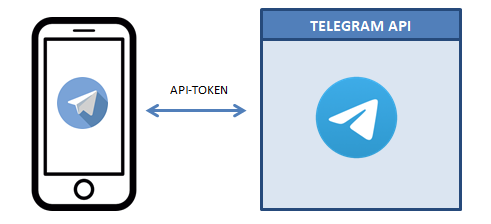
\includegraphics[scale=0.35]{images/36}
	\caption{Primera medida de seguridad}
	\label{img:seg1}
\end{figure}

Esta es la medida que nos aporta la aplicación de telegram para controlar el usuario que pueda administrar dicho bot.

El \texttt{API token} no permite la gestión del bot, pero por ahora si está permitido poder utilizar dicho bot y acceder a su conjunto de funcionalidades, por lo que esto sería un potencial riesgo.

Para prevenir este posible riesgo se ha implementado una segunda medida.

\textbf{Segunda medida: Lista blanca de usuarios}

Esta medida se basa en la implementación de una lista blanca que contiene los identificadores únicos de los usuarios que tienen permiso para utilizar el bot. Esta lista blanca está ubicada en el servicio del bot de telegram, y almacena los identificadores y nombres de usuario permitidos.

\begin{figure}[h]
	\centering
	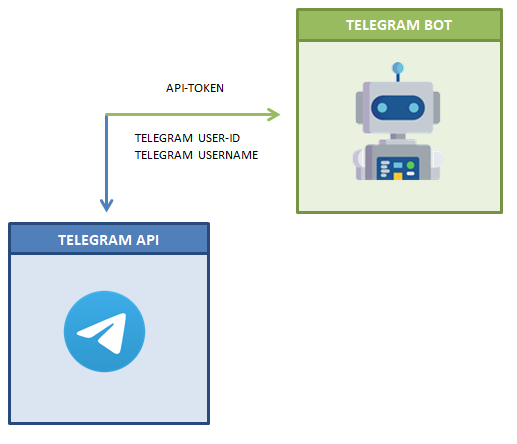
\includegraphics[scale=0.5]{images/37}
	\caption{Segunda medida de seguridad: Lista blanca de usuarios}
	\label{img:seg2}
\end{figure}

Con esta segunda medida, podemos permitir a los usuarios que queramos que tengan acceso a dicha información. Un ejemplo de esta lista blanca es el siguiente:

\vspace{-0.5cm}

\begin{verbatim}
  allowed_users = {
  				    'users':
		                 [
		                   {'id': telegram_user_id, 'username': telegram_username}, 
		                   {'id': bot_user_id, 'username': bot_username}
		                 ]
	              }
\end{verbatim}

\vspace{-0.5cm}


Si un usuario no permitido accede al bot e intenta utilizarlo se le mostrará el siguiente mensaje:

\vspace{-0.5cm}

\begin{verbatim}
You have not permission to access to this content
\end{verbatim}

\vspace{-0.5cm}

También, es importante destacar, que la \textbf{información} que viaja desde que el usuario accede a telegram, hasta que llega al servicio del bot de telegram \textbf{va cifrada}.

Las medidas aplicadas anteriormente sirven para controlar el acceso por parte de la aplicación de telegram, pero ¿y si alguna aplicación externa no autorizada intenta acceder a la \texttt{API} principal?

\texttt{Tercera medida: Autenticación usuario-contraseña}

El tercer mecanismo se basa en restringir el acceso a la \texttt{API} principal de la aplicación a través de una autenticación mediante usuario y contraseña. Esta autenticación la proporciona el módulo \texttt{authentication}, y se basa en comprobar si las credenciales de acceso son correctas,y por lo tanto, la \texttt{API} responderán a las peticiones recibidas.

Estas credenciales de acceso son necesarias para todos los servicios que quieran interactuar con la API, por lo tanto, deben de ser especificadas en el archivo de configuración \texttt{ 	authentication.yml} como se muestra a continuación:

\vspace{-0.5cm}

\begin{verbatim}
---

authentication:
    user: user
    password: sha256$tazHE31s$b4b54292237636e798e407dc935651f9af64a

\end{verbatim}

\vspace{-1cm}

Nótese que la contraseña está cifrada utilizando el algoritmo \texttt{sha256}. Para poder generar este hash, se ha proporcionado un script llamado \texttt{generate\_hash\_password.py} (ubicado en el directorio tools) para poder introducir la contraseña deseada, y se nos devuelve el hash de la contraseña.

En la siguiente figura, podemos observar como todos los servicios interaccionan con la \texttt{API} mediante un usuario y contraseña (menos con los módulos que los importa directamente).

\newpage

\begin{figure}[h]
	\centering
	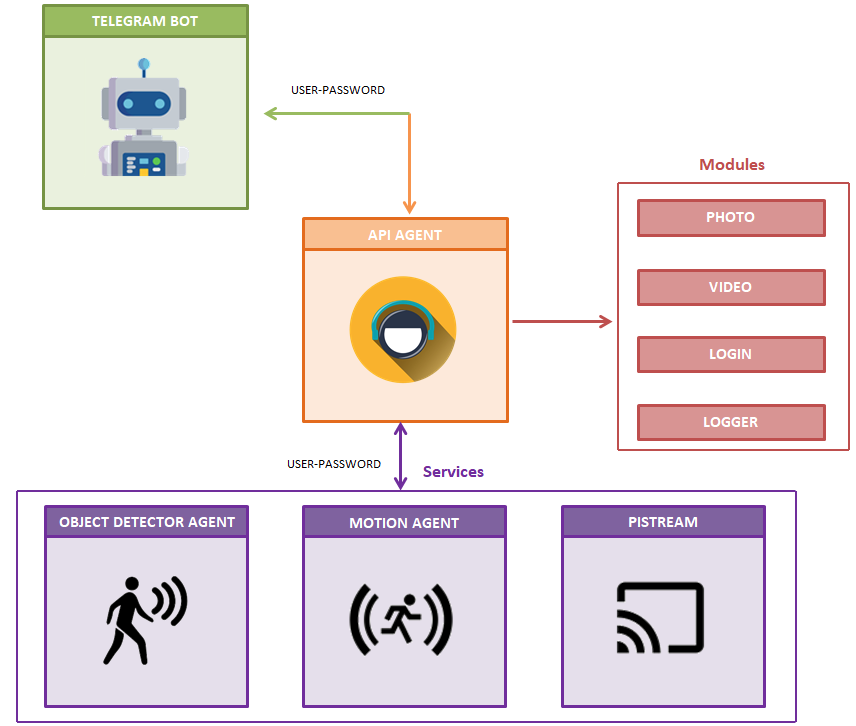
\includegraphics[scale=0.5]{images/38}
	\caption{Tercera medida de seguridad: Usuario y contraseña}
	\label{img:seg3}
\end{figure}

\subsection{Interfaz de usuario}

Para facilitar la interacción del usuario con la aplicación y mejorar su experiencia de usuario, se ha realizado un diseño de interfaz mediante botones e iconos (interfaz soportada por la API de telegram) utilizando los llamados 'Callback buttons` \cite{refx1}. Cuando un usuario pulsa estos botones, no se envía ningún mensaje al chat, sino que en su lugar el bot recibe una consulta que es manejada y respondida con una acción.

El diseño propuesto se basa en un modelo jerárquico, donde podremos ir realizando una navegación entre menús partiendo del menú principal.

Este diseño es el siguiente:

\textbf{AQUÍ VA EL DISEÑO DE LA INTERFAZ DE USUARIO} 

\newpage

Su implementación se basa en realizar un menú con un conjunto de botones con los que poder navegar. Por ejemplo, la siguiente figura muestra el menú principal, donde se puede acceder al conjunto de funcionalidades de la aplicación.

\begin{figure}[h]
	\centering
	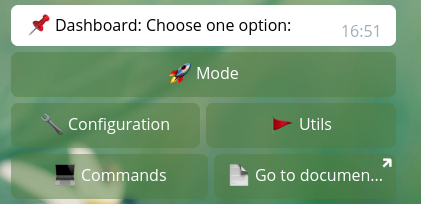
\includegraphics[scale=0.8]{images/42}
	\caption{Menú principal de la aplicación}
\end{figure}

En la sección de \textit{Mode} se podrá acceder al conjunto de acciones relacionados modos de uso de la aplicación, en \textit{Configuration} se podrá acceder al conjunto de opciones para configurar la cámara \ldots
Por ejemplo, si pulsamos el botón de \textit{Mode} se podrá acceder al conjunto de funcionalidades relacionadas.

\begin{figure}[h]
	\centering
	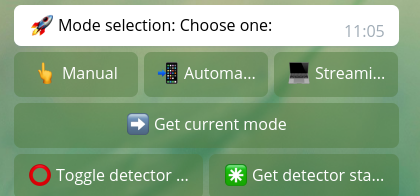
\includegraphics[scale=0.8]{images/39}
	\caption{Menú Mode}
\end{figure}

La implementación de esta interfaz se puede comprobar en este \href{https://github.com/jmv74211/TFM_security_system_PI/blob/master/src/agents/telegram_bot.py#L972}{enlace}.

\begin{tabular}{|p{15.5cm}|}
	
	\hline
	
	\textit{ \textbf{*Nota:} Para más información, todo este conjunto de botones y funcionalidades serán explicados en la guía de usuario de la sección X. }
	\\
	\hline
	
\end{tabular}

\newpage

\subsection{Descripción de archivos y directorios}

La aplicación \texttt{SIVIRA} está compuesta por una serie de archivos y directorios que implementan y ejecutan el conjunto de servicios del sistema de videovigilancia.

Todos estos archivos y directorios están disponibles en el repositorio oficial del proyecto en Github \cite{ref1}.

\begin{figure}[h]
	\centering
	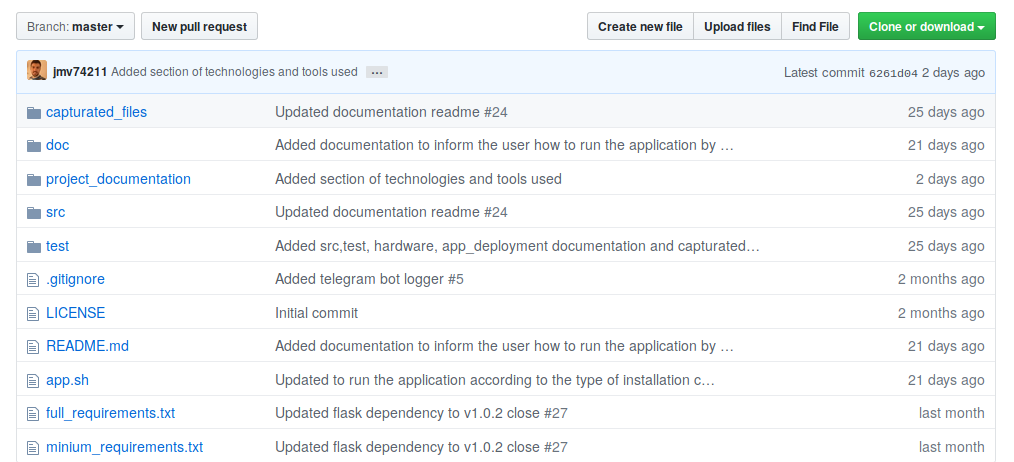
\includegraphics[scale=0.5]{images/43}
	\caption{Repositorio de Github del proyecto SIVIRA}
\end{figure}

A continuación, se explicará cómo se ha organizado todos estos archivos y directorios, junto con una breve descripción sobre el objetivo de cada uno.

\textbf{Capturated\_files}

Este directorio está destinado a almacenar el conjunto de archivos de imágenes y vídeo generados por el sistema de videovigilancia. Su estructura es la siguiente:

\tikzstyle{every node}=[draw=black,thick,anchor=west]
\tikzstyle{selected}=[draw=red,fill=red!30]
\tikzstyle{optional}=[dashed,fill=gray!50]
\begin{tikzpicture}[%
  grow via three points={one child at (0.5,-0.7) and
  two children at (0.5,-0.7) and (0.5,-1.4)},
  edge from parent path={(\tikzparentnode.south) |- (\tikzchildnode.west)}]
  \node {SIVIRA\_APP}
    child { node {capturated\_files}
		  child { node {alerts}
		  		child { node {false\_positive}}
		  }
		  child [missing] {}	
          child { node {photos}}
          child { node {videos}}
          child { node {README.md}}     
    }
    child [missing] {}	
    child [missing] {}	
    child [missing] {}	
    child [missing] {}	
    child [missing] {}	
    child { node {\ldots}};
   
\end{tikzpicture}

Se compone de los siguientes elementos:

\vspace{-0.5cm}

\begin{itemize}
\item \textbf{alerts}: Directorio donde se almacenan todos los archivos generados mediante alertas (capturas o grabaciones automáticos tras ser activado el sensor de movimiento).

	\begin{itemize}
	\item \textbf{false\_positive}: Directorio donde serán almacenados todos los archivos generados tras ser activado el sensor de movimiento y que el agente detector de objetos ha filtrado tras comprobar que no hay ninguna persona en dichas fotos.
	\end{itemize}

\item \textbf{photos}: Directorio donde se almacenan todas las fotos capturadas de forma manual.

\item \textbf{videos}: Directorio donde se almacenan todas los vídeos capturados de forma manual.

\item \textbf{Readme.md}: Archivo de documentación para el repositorio.

\end{itemize}

\textbf{Capturated\_files}

\newpage

\subsection{Test de la aplicación}